\documentclass[a4paper,10pt]{report}

\def\packagepath{../../../preambule}   % path du package princial
\usepackage{\packagepath/preambule}    % utilisation du fichier de configuration

\def\level{BTS }              % Classe
\def\course{CIEL 1}              % Matière
\def\eval{Probabilités discrètes}

\def\visibleornot{visible}    % visible or invisible
\def\documentpath{./Sources_Latex}
\def\date{Lundi 09 Février 2026}
\renewcommand{\arraystretch}{1}  % Ecart dans les tableau

\def\ptsexoA{0}
\def\ptsexoB{6}
\def\ptsexoC{4}
\def\ptsexoD{4}
\def\ptsexoE{1}
\def\ptsexoF{1}
\def\ptsexoG{2}
\def\ptsexoH{1}
\def\ptsexoI{2}
\def\ptsexoJ{2}
\def\ptsexoK{1}

\def\ptstotal{\ptsexoA+\ptsexoB}

\usepackage{hyperref}

\usetikzlibrary{shapes, arrows, positioning}
\usetikzlibrary{shapes.geometric, arrows, positioning, decorations.pathreplacing}

\tikzstyle{etat} = [draw, rounded corners=15pt, minimum width=2.5cm, minimum height=1.2cm, text centered, font=\bfseries]
\tikzstyle{nouveau} = [etat, fill=blue!40]
\tikzstyle{pret} = [etat, fill=green!60]
\tikzstyle{elu} = [etat, fill=yellow!60]
\tikzstyle{bloque} = [etat, fill=red!60]
\tikzstyle{termine} = [etat, fill=white]
\tikzstyle{fleche} = [thick, ->, >=stealth]

\usepackage{float} % Permet d'utiliser [H]
\usepackage[T1]{fontenc}
\begin{document}

%%%%%%%%%%%%%%%%%%%%%%%%%%%%%%%%%%%%%%%%%%%%%%%%%%ù

%\PageGardeSujetBac[Matiere = Numérique et Sciences Informatiques,
%                  Session = 2025,
%                  AffJour=false,
%                  Duree = {3 heures 30},
%                  DernierePage = \pageref{LastPage},
%                  ModeExamen=false
%                  ]
\renewcommand{\labelitemi}{\textbullet} %pour éviter les tirets dans les "itemize" qui apportent confusion avec le signe moins.
%% Début page de garde style BAC

   %%%%%%%%%%%%%%%%%%%%%%%%%%%%%%%%%%%%%%%%%%%%%%%%%%%%%%%%
%\PageGardeSujetBac[clés]

\pagestyle{DS_FP}          % Feuille de style fancy
\fancyhead[L]{\level -- \course}
\fancyhead[C]{\eval}
\NomPrenomNote{}

\exods{\ptsexoA}

\bigskip

\textbf{Contexte:}

\medskip

Une entreprise de composants électroniques produit des transistors. Chaque transistor peut provenir de deux chaînes de production : la chaîne A et la chaîne B. On suppose que :
\begin{itemize}
    \item 55\% des transistors proviennent de la chaîne A
    \item 45\% des transistors proviennent de la chaîne B
\end{itemize}


De plus, on constate que:
\begin{itemize}
    \item Un transistor issu de la chaîne A a 3\% de chance d'être défectueux
    \item Un transistor issu de la chaîne B a 8\% de chance d'être défectueux
\end{itemize}

On notera :
\begin{itemize}
    \item $A$ : l'événement "le transistor provient de la chaîne A"
    \item $\overline{A}$ : l'événement "le transistor provient de la chaîne B"
    \item $D$ : l'événement "le transistor est défectueux"
\end{itemize}


\medskip

\fbox{PARTIE A -- Probabilités conditionnelles}

\medskip

\begin{enumerate}[resume]

\begin{minipage}{0.62\linewidth}
    \item Compléter l'arbre des probabilités suivants avec les probabilités correspondantes.
   
    \item Calculer la probabilité d'obtenir un transistor provenant de la chaîne A et défectueux.
    \begin{answer}{1}{2} 
    $P(A\cap D)=P(A)\times P_A(D)=0.55\times 0.03=0.0165$
    \end{answer}
\end{minipage}\hfill
\begin{minipage}{0.36\linewidth}
    \begin{center}
        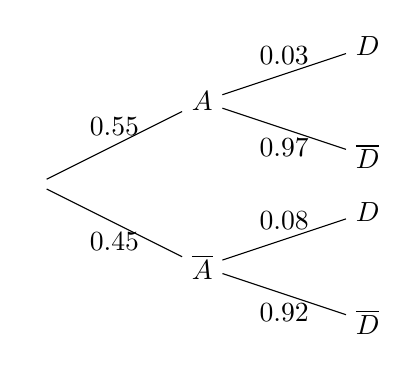
\begin{tikzpicture}[scale=0.7]
            \tikzstyle{level 1}=[level distance=3cm, sibling distance=3cm]
            \tikzstyle{level 2}=[level distance=3cm, sibling distance=2cm]
            \tikzstyle{level 3}=[level distance=3cm, sibling distance=1cm]
            \node{}[grow=right]
            child{node{$\overline{A}$}
                child{node{$\overline{D}$} edge from parent node[below]{$0.92$}}
                child{node{$ D$} edge from parent node[above]{$0.08$}}
                edge from parent node[below]{$0.45$}}
            child{node{$ A$}
                child{node{$\overline{D}$} edge from parent node[below]{$0.97$}}
                child{node{$ D$} edge from parent node[above]{$0.03$}}
                edge from parent node[above]{$0.55$}};
                \end{tikzpicture}	
            \end{center}
\end{minipage}




    
    %\item Calculer $P(\overline{A}\cap B)$ et donner une interprétation dans le cadre de l'énoncé.
    
    %\begin{answer}{1}{1.5}    \end{answer}
    
    \item Montrer que la probabilité qu'un transistor soit défectueux est de 0.0525

    \begin{answer}{1}{1.5} 
    $P(D)=P(A\cap D)+P(\overline{A}\cap D)=P(A)\times P_A(D)+P(\overline{A})\times P_{\overline{A}}(D)=0.55\times 0.03+0.45\times 0.08=0.0165+0.036=0.0525$
    \end{answer}
    
    \item Calculer la probabilité qu'un transistor provienne de la chaîne B sachant qu'il est défectueux.
    

    \begin{answer}{1}{1.5}  
    $P_D(B)=\frac{P(\overline{A}\cap D)}{P(D)}=\frac{0.45 \times 0.08}{0.0525}\approx 0.6857$
    \end{answer}

\end{enumerate}


\bigskip

\fbox{PARTIE B -- Loi binomiale}

\medskip

On vérifie la qualité des transistors en prélevant des lots de 200 transistors. On admet que la probabilité qu'un transistor soit défectueux est de 0.053. On suppose que le fait qu'un transistor soit défectueux est indépendant des autres.

On appelle X la variable aléatoire qui compte le nombre de transistors défectueux dans un lot de 200 transistors.

\begin{enumerate}[resume]
    \item Montrer que la variable aléatoire $X$ suit une loi binomiale dont on déterminera les paramètres.
    \begin{answer}{1}{4.5}  
    \begin{itemize}
        \item Choisir un transistor est une expérience aléatoire à deux issues:
        \item \begin{itemize}
            \item $S$: Succès: le transistor est défectueux, avec une probabilité de 0.053
            \item $\overline{S}$: Échec: le transistor est conforme, avec une probabilité de 0.
        \end{itemize}\
        \item Cette expérience aléatoire est répétée 200 fois de manière indépendante.
        \item La variable aléatoire $X$ compte le nombre de succès (transistors défectueux) dans ces 200 répétitions.
        \item Par conséquent, $X$ suit une loi binomiale de paramètres $n=200$ et $p=0.053$.
    \end{itemize}
    \end{answer}
    
    \item Déterminer la valeur de l'espérance de $X$ et interpréter ce résultat dans le contexte de l'énoncé.
        \begin{answer}{1}{2} 
        
        $E(X)=n\times p=200\times 0.053=10.6$

        Interprétation: En moyenne, on s'attend à trouver environ 10.6 transistors défectueux dans un lot de 200 transistors.
        \end{answer}

    \item Déterminer la probabilité d'obtenir au maximum 15 transistors défectueux dans un lot de 200 transistors. (à $10^{-4}$ près)
    \begin{answer}{1}{2}    

    En utilisant une calculatrice ou un logiciel de calcul de probabilités binomiales, on trouve que $P(X\leq 15)\approx 0.9326$ (à $10^{-4}$ près).

    \end{answer}

    

    \item Déterminer la probabilité d'obtenir entre 10 et 20 transistors défectueux (inclus) dans un lot de 200 transistors. (à $10^{-4}$ près)
    \begin{answer}{1}{2}  
    
    
    En utilisant une calculatrice ou un logiciel de calcul de probabilités binomiales, on trouve que 
    
    $P(10\leq X\leq 20)\approx 0.6173$ (à $10^{-4}$ près).
    \end{answer}

\end{enumerate}

\medskip




\fbox{PARTIE C -- On suppose maintenant qu'on fabrique une série de n transistors. }

\medskip

\begin{enumerate}[resume]

\begin{minipage}{0.59\linewidth}
    \item Exprimer en fonction de n la probabilité que tous les transistors de la série soient conformes (non défectueux).
\end{minipage}\hfill
\begin{minipage}{0.39\linewidth}
    \begin{answer}{1}{1.5} $P_{tous\, conformes} = (1-0.053)^n = 0.947^n$   \end{answer}

\end{minipage}

\begin{minipage}{0.59\linewidth}
    \item En déduire le nombre minimum de transistors qu'il faut fabriquer pour que la probabilité d'avoir au moins un transistor défectueux soit supérieure à 0.9.
\end{minipage}\hfill
\begin{minipage}{0.39\linewidth}
    \begin{answer}{1}{3} 
        
        $P(X>=1)=1-P(X=0)=1-0.947^n$
        
        $n_{minimum}= 43$  \end{answer}

\end{minipage}

\appelprof{}

\end{enumerate}


\end{document}
